


\section{Unemployment}
\label{sec-1}







  


This \texttt{zoo} object can be directly displayed with the \texttt{xyplot.zoo} method. 


\lstset{language=R}
\begin{lstlisting}
xyplot(unemployUSA, superpose=TRUE,
       par.settings=custom.theme.2,
       auto.key=list(space='right'))
\end{lstlisting}

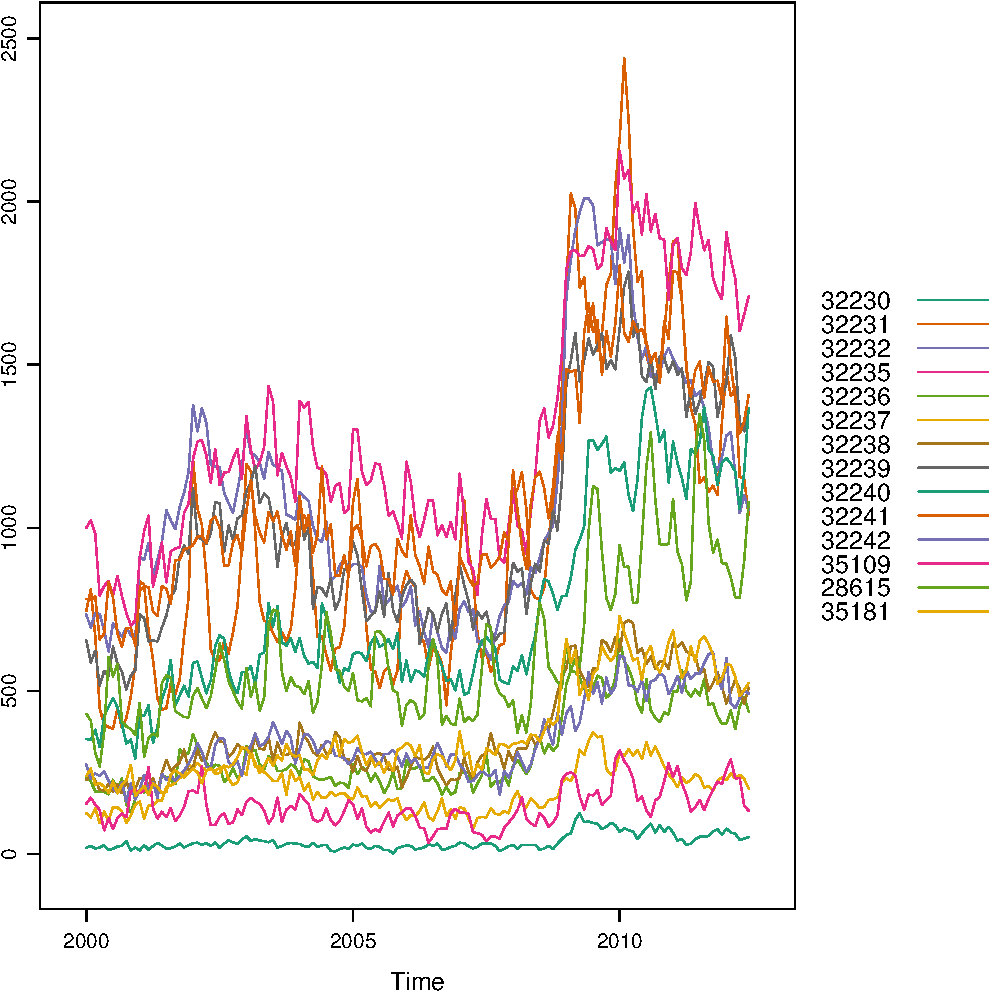
\includegraphics[width=.9\linewidth]{/home/oscar/Dropbox/chapman/book/figs/unemployUSAxyplot.pdf}


This graphical output is not very useful: the legend is confusing with
too many items; the vertical scale is dominated by two series with the
bulk of the series buried in the lower part of the scale; the trend,
variations and structure of the total and the individual contributions
cannot be deduced from this graph.

A suitable improvement is to display the multivariate time series as a
set of stacked colored polygons with a time line at the bottom: the
ThemeRiver.


\cite{Havre.Hetzler.ea2002} The ThemeRiver visualization displays
time series with stacked colored polygons in the context of a time
line at the bottom of the figure. This combination allows a user
to discern patterns in individual themes and among multiple themes
relative to time. These patterns may reveal trends, relationships,
anomalies, and structure in the data.



The \texttt{xyplot} function displays information according to the class
of its first argument (methods) and to the \texttt{panel} function. We
will use the \texttt{xyplot.zoo} method (equivalent to the \texttt{xyplot.ts}
method) with a new custom \texttt{panel} function.
This new function has four main arguments, three of them calculated by
\texttt{xyplot} (\texttt{x}, \texttt{y} and \texttt{groups}) and a new one, \texttt{origin}. Of
course, it includes the \texttt{...} argument to provide additional
arguments.

\index{Panel function}
\index{superpose.polygon@\texttt{superpose.polygon}}
\index{trellis.par.get@\texttt{trellis.par.get}}
\index{apply@\texttt{apply}}
\index{sapply@\texttt{sapply}}
\index{unstack@\texttt{unstack}}
\index{panel.text@\texttt{panel.text}}
\index{panel.polygon@\texttt{panel.polygon}}

\lstset{language=R}
\begin{lstlisting}
panel.flow <- function(x, y, groups, origin, ..., pos=4){
  dat <- data.frame(x=x, y=y, groups=groups)
  nVars <- nlevels(groups)
  groupLevels <- levels(groups)

  yWide <- unstack(dat, y~groups)

  ##Havre.Hetzler.ea2002
  if (origin=='themeRiver') origin= -1/2*rowSums(yWide)
  else origin=0 

  yWide <- cbind(origin=origin, yWide)
  yCumSum <- t(apply(yWide, 1, cumsum))
  Y <- as.data.frame(sapply(seq_len(nVars),
                            function(iCol)c(yCumSum[,iCol+1],
                                            rev(yCumSum[,iCol]))))
  names(Y) <- levels(groups)
  y <- stack(Y)$values

  xWide <- unstack(dat, x~groups)
  x <- rep(c(xWide[,1], rev(xWide[,1])), nVars)

  groups <- rep(groups, each=2)

  superpose.polygon <- trellis.par.get("superpose.polygon")

  col = superpose.polygon$col
  border = superpose.polygon$border 
  lwd = superpose.polygon$lwd 

  for (i in seq_len(nVars)){
    xi <- x[groups==groupLevels[i]]
    yi <- y[groups==groupLevels[i]]
    panel.polygon(xi, yi, border=border,
                  lwd=lwd, col=col[i])
    N <- length(xi)/2
    panel.text(xi[N], (yi[N]+yi[N+1])/2,
               labels=groupLevels[i],
               col=col[i], pos=pos, ...)
  }
}
\end{lstlisting}

The first step is to create a \texttt{data.frame} with the coordinates
and with the \texttt{groups} factor. The value and number of its levels
will be used in the main step of this \texttt{panel} function.With this
\texttt{data.frame} we have to calculate the \texttt{y} and \texttt{x} coordinates for
each group to get an stacked set of polygons.

This \texttt{data.frame} is in the \emph{long} format, with a row for each
observation where the \texttt{group} column identifies the
variable. Thus, it has to transformed to the \emph{wide} format, with a
column for each variable. With the \texttt{unstack} function a new
\texttt{data.frame} is produced, whose columns are defined according to
the formula \texttt{y \textasciitilde{} groups} and with a row for each time
position. The stack of polygons is the result of the cumulative
sum of each row (\texttt{apply(yWide, 1, cumsum)}). The origin of this sum
is defined with the corresponding \texttt{origin} argument: with =origin
= `themeRiver'= the polygons are arranged in a symmetric way.

Each column of this matrix of cumulative sums defines the \texttt{y}
coordinate of each variable (where \texttt{origin} is now the first
variable). The polygon of each variable is comprised between this
curve (\texttt{iCol+1}) and the one of the previous variable (\texttt{iCol}). In
order to get a closed polygon, the coordinates of the inferior
limit are in reverse order. This new \texttt{data.frame} (\texttt{Y}) is in the
\emph{wide} format, but \texttt{xyplot} requires the information in the \emph{long}
format: the \texttt{y} coordinates of the polygons are extracted from the
\texttt{values} column of the \emph{long} version of this \texttt{data.frame}.

The \texttt{x} coordinates are produced in easier way. Again, \texttt{unstack}
produces a \texttt{data.frame} with column for each variable and a row
for each time position but now, since the \texttt{x} coordinates are the same
for the set of polygons, the corresponding vector is constructed
directly with a combination of concatenation a repetition.

Finally, the \texttt{groups} vector is produced repeating each element of
the column of the original \texttt{data.frame} (\texttt{dat\$groups}) twice to
account for the forward and reverse curves of the corresponding
polygon.

The last step before displaying the polygons is to acquire the
graphical settings. The information retrieved with
\texttt{trellis.par.get} is transferred to the corresponding arguments of
\texttt{panel.polygon}.

Everything is ready for constructing the polygons. With a \texttt{for}
loop the coordinates of the corresponding group are extracted from
the \texttt{x} and \texttt{y} vectors. A polygon is displayed with
\texttt{panel.polygon} and labelled with \texttt{panel.text} (where the labels
are the \texttt{levels} of the original \texttt{groups} variable,
\texttt{groupLevels}). Both the polygon and its label share the same
color (\texttt{col[i]}).

With this panel function, \texttt{xyplot} will display a set of stacked
polygons corresponding to the multivariate time series. However,
the graphical window is not large enough and part of the polygons
fall out of it. Why?



\lstset{language=R}
\begin{lstlisting}
library(colorspace)

nCols <- ncol(unemployUSA)
pal <- rainbow_hcl(nCols, c=70, l=75, start=30, end=300)
myTheme <- custom.theme(fill=pal, lwd=0.4)

xyplot(unemployUSA, superpose=TRUE, auto.key=FALSE,
       panel=panel.flow, origin='themeRiver',
       par.settings=myTheme, cex=0.4, offset=0,
       scales=list(y=list(draw=FALSE)))
\end{lstlisting}

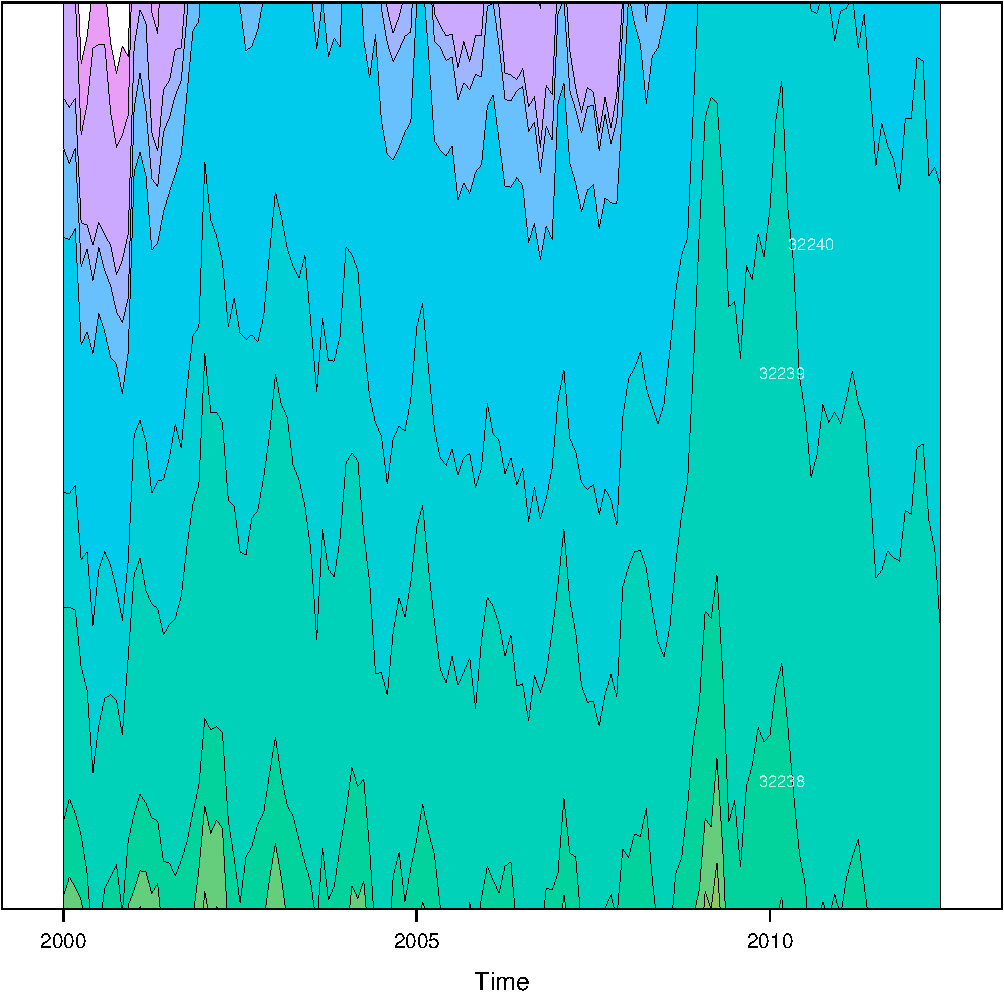
\includegraphics[width=.9\linewidth]{/home/oscar/Dropbox/chapman/book/figs/ThemeRiverError.pdf}

The problem is that \texttt{lattice} makes a preliminary estimate of the
window size using a default \texttt{prepanel} function which is unaware
of the internal calculations of our new \texttt{panel.flow} function. The
solution is to define a new \texttt{prepanel.flow} function. The input
arguments and first lines are exactly the same as in
\texttt{panel.flow}. The output is a list whose elements are the limits
for each axis (\texttt{xlim} and \texttt{ylim}), and the sequence of differences
(\texttt{dx} and \texttt{dy}) which can be used for the aspect and banking
calculations. The limits of the x-axis are defined with the range
of the time index, while the limits of the y-axis are calculated
with the minimum of the first column of \texttt{yyy} (the origin line)
and with the maximum of its last column (the upper line of the
cumulative sum).


\lstset{language=R}
\begin{lstlisting}
prepanel.flow <- function(x, y, groups, origin,...){
  dat <- data.frame(x=x, y=y, groups=groups)
  nVars <- nlevels(groups)
  groupLevels <- levels(groups)
  yWide <- unstack(dat, y~groups)
  if (origin=='themeRiver') origin= -1/2*rowSums(yWide)
  else origin=0
  yWide <- cbind(origin=origin, yWide)
  yCumSum <- t(apply(yWide, 1, cumsum))

  list(xlim=range(x),
       ylim=c(min(yCumSum[,1]), max(yCumSum[,nVars+1])),
       dx=diff(x),
       dy=diff(c(yCumSum[,-1])))
}
\end{lstlisting}

The output of \texttt{xyplot} using both the panel and prepanel functions
is displayed in the figure fig:unemployUSAThemeRiver.


\lstset{language=R}
\begin{lstlisting}
xyplot(unemployUSA, superpose=TRUE, auto.key=FALSE,
       panel=panel.flow, prepanel=prepanel.flow,
       origin='themeRiver', scales=list(y=list(draw=FALSE)),
       par.settings=myTheme, cex=0.4, offset=0)
\end{lstlisting}

\begin{figure}[htb]
\centering
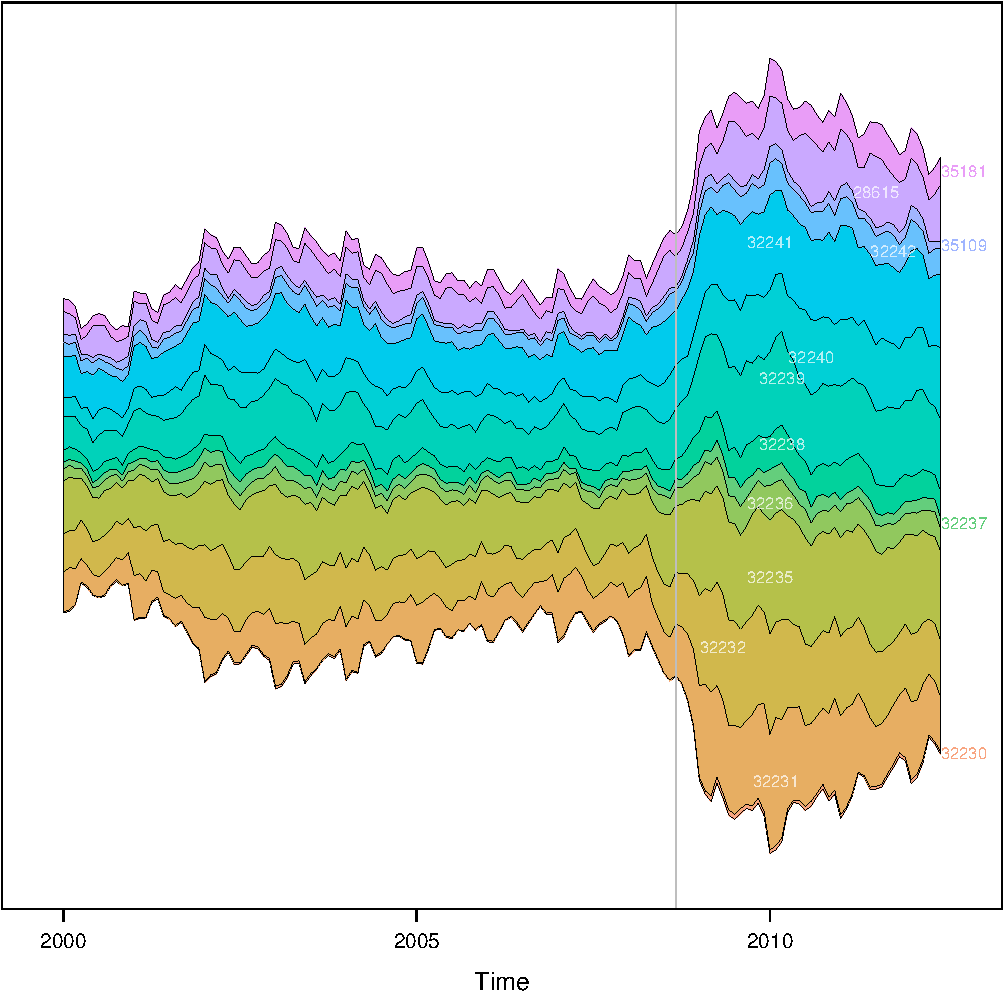
\includegraphics[width=.9\linewidth]{/home/oscar/Dropbox/chapman/book/figs/unemployUSAThemeRiver.pdf}
\caption{\label{fig:unemployUSAThemeRiver}Theme River of unemployment at USA}
\end{figure}
